\documentclass[letterpaper,12pt]{amsart}

\setlength{\evensidemargin}{-0.0in}
\setlength{\oddsidemargin}{-0.0in}
\setlength{\textwidth}{6.4in}

\usepackage[utf8]{inputenc}
\usepackage{amsmath}
\usepackage{amssymb}
\usepackage{enumerate}
%\usepackage{mathpazo}
\usepackage{relsize}
\usepackage{mathtools}
\usepackage{mathrsfs}
\usepackage{verbatim}

\usepackage{hyperref}
\hypersetup{
    colorlinks=true,
    linkcolor=blue,
    filecolor=magenta,      
    urlcolor=blue,
}

\usepackage{tikz}
\usetikzlibrary{matrix,arrows}

\usepackage{fancyhdr}
\pagestyle{fancy}
\lhead{Gieseker-to-Uhlenbeck}
\rhead{Tuomas Tajakka}
%\cfoot{}
\rfoot{}
\renewcommand{\headrulewidth}{0.4pt}

\usepackage{amsthm}

\newtheorem{thm}{Theorem}[section]
\newtheorem{lem}[thm]{Lemma}
\newtheorem{prop}[thm]{Proposition}
\newtheorem{cor}[thm]{Corollary}
\newtheorem{expl}[thm]{Example}
\newtheorem{defn}[thm]{Definition}

\theoremstyle{remark}
\newtheorem{rmk}[thm]{Remark}
\newtheorem{exer}[thm]{Exercise}

\title{Projectivity of the Gieseker moduli space via Bridgeland stability}
\author{Tuomas Tajakka}
\date{}

\usepackage{commands}


\begin{document}

\maketitle

\section{Introduction}
The purpose of this note is to provide a new proof of the classical result that the moduli space of Gieseker-semistable sheaves on a smooth, projective surface is a projective scheme. Our proof is based on viewing the Gieseker moduli space as a Bridgeland moduli space and relies on the theory of line bundles on Bridgeland moduli spaces developed by Bayer and Macr\`i \cite{BM} together with the author's earlier result that the Uhlenbeck compactification is projective \cite{t}. Our method has the benefit of avoiding the use of GIT, which as of now is unavailable in general for constructing moduli spaces of Bridgeland semistable objects on a surface. However, we must unfortunately restrict to the case when the rank and first Chern class are coprime.

\section{Bridgeland stability}
\subsection{Stability conditions on a surface}
In this section we recall some necessary facts about the Bridgeland stability conditions on surfaces. Instead of giving the full definition, we only outline the construction of the stability conditions relevant to us, and refer the reader to \cite{bridgeland}, \cite{bridgelandK3}, \cite{ABL13}, and \cite{MS} for a more complete discussion. Very briefly, a \textbf{(numerical) stability condition} on a smooth, projective variety $X$ is a pair $\si = (\sA, Z)$ consisting of a heart of a bounded t-structure $\sA \subs D^b(X)$ and a group homomorphism $\Kn(X) \to \C$ satisfying certain axioms, most important of which is the requirement that for every nonzero object $A \in \sA$, we have
\[ Z(A) \in \Hb = \Hh \cup \R_{<0} = \{ z \in \C \;|\; |z| > 0, \; 0 < \arg(z) \le \pi \}. \]
This lets us define a notion of stability in the abelian category $\sA$ by saying that $A \in \sA$ is \textbf{stable} (resp. \textbf{semistable}) if for every proper nonzero subobject $A' \subs A$, we have
\[ \arg(Z(A')) < \arg(Z(A)) \qquad (\mathrm{resp.} \quad \arg(Z(A')) \leq \arg(Z(A')). \]
Moreover, we say that $E \in D^b(X)$ is stable or semistable if for some $n \in \Z$, the shift $E[n]$ lies in $\sA$ and is stable or semistable. Stability conditions on $X$ are parameterized by a complex manifold $\Stab(X)$, and for a fixed numerical class $v \in \Kn(X)$, there is a locally finite wall-and-chamber decomposition in $\Stab(X)$ with the property that in each open chamber, the isomorphism classes of stable and semistable objects remain unchanged.

We now recall the standard construction of stability conditions on a surface, achieved by tilting $\Coh(X)$ with respect to the Mumford-Takemoto slope. Let $(X, H)$ be a smooth, projective, polarized surfaces over $\C$, where $H \subset X$ is a very ample divisor. For a real divisor class $B \in N^1(X)_\R$, we define the {\bf $B$-twisted slope function} on $\Coh(X)$ by
\[ \mu_B(E) = \frac{H \cdot \ch_1(E)}{H^2 \cdot \ch_0(E)} - \frac{H \cdot B}{H^2} \]
if $\rk(E) > 0$, and $\mu_B(E) = \infty$ if $\rk(E) = 0$, i.e. $E$ is a torsion sheaf. For a real number $\be$, we have a torsion pair on $\Coh(X)$ given by
\begin{align*}
    \sT_\be & = \{ E \in \Coh(X) \;|\; \mathrm{every\;semistable\;factor\;} F \mathrm{\;of\;} E \mathrm{\;satisfies\;} \mu_B(F) > \be\}, \\
    \sF_\be & = \{ E \in \Coh(X) \;|\; \mathrm{every\;semistable\;factor\;} F \mathrm{\;of\;} E \mathrm{\;satisfies\;} \mu_B(F) \le \be\},
\end{align*}
and tilting $\Coh(X)$ with respect to this torsion pair yields a heart of a bounded t-structure 
\[ \Coh^\be(X) = \langle \sF_\be[1], \sT_\be \rangle \subs D^b(X) \] 
defined as the full subcategory whose objects are precisely those $E \in D^b(X)$ fitting in an exact triangle
\begin{equation}\label{FETtriangle}
    F[1] \to E \to T, 
\end{equation}
where $F \in \sF_\be, T \in \sT_\be$. Moreover, for any $\al \in \R_{>0}$ we define a map $Z_{\al,\be}: \Kn(X) \to \C$ by setting
\begin{align*}
    Z_{\al, \be}(E) & = -\int_X e^{-(\be + i \al)H} \ch^B(E) \\
    & = \frac{\al^2 - \be^2}{2} H^2 \ch^B_0(E) + \be H\cdot\ch^B_1(E) - \ch^B_2(E) \\
    & \quad  + i\al(H \cdot \ch^B_1(E) - \be H^2 \ch^B_0(E)),
\end{align*}
where
\[ \ch^B(E) = e^{-B}\cdot \ch(E) = \ch_0^B(E) + \ch_1^B(E) + \ch_2^B(E) \in A^*(X) \]
is the $B$-twisted Chern character of $E \in D^b(X)$.
\begin{prop}[{\cite[Corollary 2.1]{ABL13}}]
    The pair $\si_{\al,\be} = (\sA_\be, Z_{\al,\be})$ is a stability condition on $D^b(X)$.
\end{prop}
The stability conditions $\si_{\al,\be}$ are parameterized by the upper half plane $\be \in \R, \al \in \R_{>0}$. The wall-and-chamber structure in this half-plane was analyzed in \cite{maciocia}. If $v \in \Kn(X)$ is a class of positive rank, then there is a unique vertical wall at 
\[ \be_0 = \frac{H \cdot \ch_1^B(v)}{H^2 \ch_0(v)}, \] and on each side of the vertical wall, there is a nested sequence of semicircles with center on the $\be$-axis and contained in a largest semicircle. In particular, on either side of the vertical wall, there is an unbounded open chamber. The walls in the $(\al,\be)$-plane are pairwise disjoint, and so there is no further wall-and-chamber decomposition within each wall.
\begin{center}
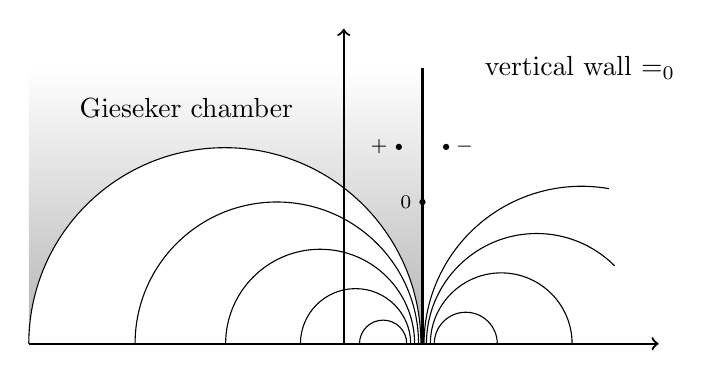
\begin{tikzpicture}
\shadedraw[bottom color=black!30!white,top color=white,draw=white] (-4,0) arc (180:0:2.49) -- (0,0) -- (1,0) -- (1,3.5) -- (-4,3.5);

\draw[thick,->] (-4,0) -- (4,0) node[anchor=south east] {$\be$};
\draw[thick,->] (0,0) -- (0,4) node[anchor=north west] {$\al$};

\draw[thick] (1,0) -- (1,3.5);

\draw[] (0.98,0) arc (0:180:2.49);
\draw[] (0.95,0) arc (0:180:1.8);
\draw[] (0.9,0) arc (0:180:1.2);
\draw[] (0.85,0) arc (0:180:0.7);
\draw[] (0.8,0) arc (0:180:0.3);

\draw[] (1.02,0) arc (180:80:2);
\draw[] (1.05,0) arc (180:45:1.4);
\draw[] (1.1,0) arc (180:0:0.9);
\draw[] (1.15,0) arc (180:0:0.4);

\draw (-2,3) node {Gieseker chamber};
\draw (3,3.5) node {vertical wall $\be = \be_0$};
\fill (1,1.8) circle (0.04) node[anchor=east] {$\si_0$};
\fill (0.7,2.5) circle (0.04) node[anchor=east] {$\si_+$};
\fill (1.3,2.5) circle (0.04) node[anchor=west] {$\si_-$};
\end{tikzpicture}
\end{center}

When $\si_0 \in \Stab(X)$ lies on the vertical wall for $v$, the stable and semistable objects of class $v$ can be classified as follows. The heart $\sA_{\be_0}$ contains no objects of class $v$, so it is more natural to consider the heart $\sA_{\be_0}[-1]$ whose objects fit in a triangle
\begin{equation}\label{FET2}
    F \to E \to T[-1]
\end{equation}
analogous to \eqref{FETtriangle}.
\begin{prop}[{\cite[Proposition 2.2]{t}}]
    Let $v \in \Kn(X)$ be a class with $\rk(v) > 0$, and let $\si_0 \in \Stab(X)$ be class on the vertical wall for $v$. An object $E \in \sA_{\be_0}[-1]$ of class $v$ is
    \begin{itemize}
        \item \textit{semistable} if in the triangle \eqref{FET2}, the sheaf $F$ is $\mu_B$-semistable and the sheaf $T$ is 0-dimensional,
        \item \textit{stable} if in \eqref{FET2}, $F$ is $\mu$-stable and locally free,
        \item \textit{polystable} if
        \[ E \cong F \oplus \left(\bigoplus_{i=1}^n \Oh_{p_i}[-1] \right), \]
        where $F$ is a $\mu$-polystable locally free sheaf and $p_i \in X$ are closed points.
    \end{itemize}
\end{prop}
The open unbounded chamber left of the vertical wall is called the \textbf{Gieseker chamber} for the following reason.
\begin{prop}
    Let $v \in \Kn(X)$ be a class with $\rk(v) > 0$ and let $\si_+ = (\sA_\be, Z_{\al,\be} \in \Stab(X)$ be in the Gieseker chamber, that is, $\be < \be_0$. An object $E \in \sA_\be$ of class $v$ is $\si_+$-stable (resp. $\si_+$-semistable, $\si_+$-polystable) if in the triangle \eqref{FETtriangle}, the sheaf $T$ is Gieseker-stable (resp. Gieseker-semistable, Gieseker-polystable) and $F = 0$.
\end{prop}
Finally, the unbounded chamber right of the vertical wall is the \textbf{dual Gieseker chamber}:
\begin{prop}
    Let $v \in \Kn(X)$ be a class with $\rk(v) > 0$ and let $\si_- = (\sA_\be, Z_{\al,\be} \in \Stab(X)$ be in the dual Gieseker chamber, that is, $\be > \be_0$. An object $E \in \sA_\be[-1]$ of class $v$ is $\si_-$-stable (resp. $\si_-$-semistable, $\si_-$-polystable) if and only if the derived dual $R\sHom(E, \Oh_X)$ is a Gieseker-stable (resp. Gieseker-semistable, Gieseker-polystable) sheaf. {\color{red} Make a more precise statement, including how the numerical invariants change.}
\end{prop}

\subsection{Moduli spaces of semistable objects}
For a stability condition $\si = (\sA, Z)$ on $X$, we denote the moduli stack of $\si$-semistable objects in $\sA$ by $\sM^\si_X(v)$. By \cite{toda08}, when $\si$ lies in the connected component containing the Gieseker chamber, the stack $\sM^\si_X(v)$ is a quasi-compact, universally closed, open substack of the universally glueable complexes constructed in \cite{lie06}. Moreover, by \cite[Theorem 7.25]{AHLH}, the stack $\sM^\si_X(v)$ admits a good moduli space $M^\si_X(v)$ which is a proper algebraic space.

\subsection{Positive line bundles on the moduli space}
In \cite{BM}, the authors construct a natural numerical class $\sL_\si$ of line bundles on $\sM^\si(v)$ with strong positivity properties. Consider the diagram
\begin{center}
    \begin{tikzpicture}
    \matrix (m) [matrix of math nodes, row sep=1em, column sep=1em]
    { & \sE & \\
    & \sM^\si_X(v) \times X & \\
    \sM^\si_X(v) & & X \\};
    \path[dotted,-] 
    (m-1-2) edge node[auto,swap] {$ $} (m-2-2)
    ;
    \path[->] 
    (m-2-2) edge node[auto,swap] {$ p $} (m-3-1)
    (m-2-2) edge node[auto] {$ q $} (m-3-3)
    ;
    \end{tikzpicture}
\end{center}
where $\sE \in D^b(\sM^\si_X(v) \times X)$ is the universal complex. The class $\sL_\si$ is defined as the determinantal line bundle
\[ \la_\sE(w_\si) \coloneqq \det(R p_*( \sE \otimes q^* w_\si)), \]
where $w_\si \in \Kn(X)$ is the unique numerical class defined by the condition
\[ \chi(w_\si \otimes - ) = \im\left(- \frac{Z(-)}{Z(v)}\right). \]
The key property of $\sL_\si$ is the following.
\begin{thm}[{\cite[Lemma 3.3]{BM}, \cite[Lemma 5.3]{t}}]
    Let $C$ be a smooth, projective curve and let $f: C \to \sM^\si_X(v)$ be a morphism corresponding to a family $\sE' \in D^b(C \times X)$ of semistable objects. We have $\deg f^* \sL_\si \ge 0$, and $\deg f^* \sL_\si = 0$ if and only if $\sE'$ is a family of S-equivalent objects.
    
    Moreover, the class $\sL_\si$ descends to a class $L_\si$ on the good moduli space $M^\si_X(v)$ with the following properties. If $g: C \to M^\si_X(v)$ is a morphism, then $\deg g^*L_\si \ge 0$, and $\deg g^* L_\si = 0$ if and only if $g$ is a constant map.
\end{thm}

The present author's main result in \cite{t} is that when $\si_0 \in \Stab(X)$ lies on the vertical wall for $v \in \Kn(X)$, the class $L_\si$ is actually ample on $M^{\si_0}_X(v)$ and consequently $M^{\si_0}_X(v)$ is a projective scheme.

\section{Algebraic preliminaries}
Let $k$ be a field and let $(R,\frm,k)$ be a local $k$-algebra. 
\begin{lem}\label{killedbymn}
    If $Q$ is an $R$-module whose dimension over $k$ is $n < \infty$, then the ideal $\frm^n \subs R$ acts by zero on $Q$. 
\end{lem}
\begin{proof}
Since $Q$ is finite-dimensional over $k$, the descending sequence
\[ Q \supset \frm Q \supset \frm^2 Q \cdots \]
must terminate at some $\frm^d Q = \frm^{d+1} Q = \cdots$, and by Nakayama's lemma each containment until $d$ is strict and $\frm^d Q = 0$. Thus,
\[ n = \dim Q = \sum_{i=0}^{d-1} \frm^i Q/\frm^{i+1} Q \ge d. \]
\end{proof}

Assume now that $R$ an artinian, and denote $d = \dim_\C R$, and let $F$ be a free $R$-module of rank $r$, so that $F$ has dimension $d r$ over $\C$. We can view $R$ as a sheaf of algebras on $\Spec \C$, and similarly $F$ as a coherent sheaf of $R$-algebras on $\Spec \C$.
\begin{lem}\label{subgrass}
    Define a functor $(Sch_\C)^{\text{op}} \to Sets$ that to a $\C$-scheme $T \xrightarrow{\pi} \Spec \C$ associates the set of isomorphism classes of quotients
    \[ q: \pi^*F \twoheadrightarrow Q \]
    of $\pi^*R$-modules with $Q$ locally free over $\Oh_T$ of rank $n$, where two quotients $q$ and $q'$ are isomorphic if there is an isomorphism $\al: Q \to Q'$ of $\Oh_T$-modules such that $q' = q \circ \al$. The functor $\Phi$ is represented by a closed subscheme of the Grassmannian $\Gr(F, n)$ of $n$-dimensional quotients of $F$ viewed as a $\C$-vector space.
\end{lem}
\begin{proof}
    There is a natural transformation 
\end{proof}

\section{Projectivity of the Gieseker moduli space}
Let $(X, H)$ be a smooth, projective, polarized surface, and let $v \in \Kn(X)$ be a class of rank $r = \rk(v) > 0$. We make the assumption that $\gcd(\rk(v), H\cdot c_1(v)) = 1$, which implies that for a torsion-free sheaf $F \in \Coh(X)$ of class $v$, the conditions of being $\mu$-stable, $\mu$-semistable, Gieseker-stable, and Gieseker-semistable are all equivalent.

Let $\si_+, \si_0 \in \Stab(X)$ be stability conditions in the Gieseker chamber and on the vertical wall of the $(\al,\be)$-plane respectively. We have an inclusion of algebraic stacks $\sM^{\si_+}_X(v) \to \sM^{\si_0}_X(v)$ which induces a morphism
\[ f: M^{\si_+}_X(v) \to M^{\si_0}_X(v) \]
of their good moduli spaces. By \cite[Theorem 1.1]{t}, the moduli space $M^{\si_0}_X(v)$ is projective and the line bundle $L_{\si_0} \in \Pic(M^{\si_0}_X(v))$ is ample. Our main result is the following.
\begin{thm}\label{giesproj}
    The line bundle $L_{\si_+} \in \Pic(M^{\si_+}_X(v))$ is ample relative to the morphism $f: M^{\si_+}_X(v) \to M^{\si_0}_X(v)$. In particular, the moduli space $M^{\si_+}_X(v)$ is a projective scheme.
\end{thm}
Our strategy to prove Theorem \ref{giesproj} is as follows. Since $f: M^{\si_+}_X(v) \to M^{\si_0}_X(v)$ is a proper morphism from an algebraic space to a noetherian scheme, by \cite[\href{https://stacks.math.columbia.edu/tag/0D3A}{Tag 0D3A}]{stacks-project} it suffices to show that the restriction of $L_{\si_+}$ to each fiber of $f$ is ample. Now for a given closed point $s \in M^{\si_0}_X(v)$ will construct a projective scheme $S$ and a family $\sE$ of $\si_+$-stable sheaves of class $v$ parameterized by $S$ such that the induced morphism
\[ S \to \sM^{\si_+}_X(v) \to M^{\si_+}_X(v) \]
maps $S$ bijectively onto the fiber $f^{-1}(s)$. In fact, we will construct $S$ as a product of closed subschemes of Grassmannians. Using properties of the universal quotient parameterized by the Grassmannian, we will show that the pullback of the line bundle $L_{\si_+}$ to $S$ is ample, and conclude that $L_{\si_+}|_{f^{-1}(s)}$ is ample on $f^{-1}(s)$.

To carry out this strategy, suppose that the point $s \in M^{\si_0}_X(v)$ corresponds to the object
\[ F \oplus \bigoplus_{i=1}^m \Oh_{x_i}^{\oplus n_i}[-1] \in D^b(X), \]
where $F \in \Coh(X)$ is a $\mu$-stable locally free sheaf, the $x_i \in X$ are closed points, and $n_i \in \N$. The points of the fiber $f^{-1}(s) \subs M^{\si_+}_X(v)$ are in bijection with torsion-free sheaves $E \in \Coh(X)$ such that 
\begin{itemize}
    \item $E^{\vee\vee} \cong F$, 
    \item the quotient $E^{\vee\vee}/E$ has length $n_i$ at $x_i$.
\end{itemize}
Said differently, the fiber parameterizes isomorphism classes of quotients of $F$ supported at the points $x_i$ with length $n_i$. Let $\frm_i$ denote the maximal ideal of $\Oh_i$, and set $R_i = \Oh_{X,x_i}/\frm_i^{n_i}$. By Lemma \ref{killedbymn}, any quotient of $q: F \twoheadrightarrow Q$ where $Q$ is supported at the points $x_i$ with lengths $n_i$ must factor as
\[ F \twoheadrightarrow \bigoplus_{i=1}^m F/\frm_i^{n_i} F \twoheadrightarrow Q. \]
Thus, denoting $V_i = F/\frm_i^{n_i}F$, the fiber $f^{-1}(s)$ parameterizes quotients $\oplus_i V_i$ that have length $n_i$ at $x_i$. 

Now by Lemma \ref{subgrass}, there is a scheme $S_i$ parameterizing quotients of $V_i$ of length $n_i$, and there is a quotient
\begin{equation}\label{sesi}
    V_i \otimes \Oh_{S_i} \twoheadrightarrow \sQ_i
\end{equation} 
where $\sQ_i$ is a locally free $\Oh_{S_i}$-module such that, letting $q_i: S_i \times X \to X$ denote the second projection, $\sQ_i$ has the structure of a $q^* R_i$-module. 

Let $\io_i: S_i \to S_i \times X$ denote the map given by $\io_i(s) = (s, x_i)$. Pushing the sequence \eqref{sesi} forward by $\io_i$, we obtain a quotient
\[ q_i^* V_i = V_i \otimes \Oh_{S_i} \twoheadrightarrow \io_{i,*} \sQ_i \]
of $q_i^* R_i$-modules, and hence of $\Oh_{S_i\times X}$-modules via the map $\Oh_{S_i \times X} \cong q^* \Oh_X \to q^*R_i$ of $\Oh_{S_i \times X}$-algebras. Precomposing this with the pullback of the quotient $F \twoheadrightarrow F/\frm_i^{n_i}$ along $q_i$, we obtain a quotient
\begin{equation}\label{ithquot}
    q_i^*F \twoheadrightarrow \io_{i,*} \sQ_i,
\end{equation}
and since $\io_{i,*} \sQ_i$ is locally free of finite rank as an $\Oh_{S_i}$-module, it is flat over $S_i$.

Now define $S = \prod_{i=1}^m S_i$, and let $\pi_i: S \times X \to S_i \times X$ denote the projection, and $q: S \times X \to X$ the second projection. Pulling back the map \eqref{ithquot} along $\pi_i$, we have surjections 
\[ q^* F \twoheadrightarrow \pi_i^* \io_{i,*}\sQ_i, \]
and since the sheaves $\pi_i^* \io_{i,*}\sQ_i$ have disjoint support, we obtain a short exact sequence
\begin{equation}\label{bigquotient}
    0 \to \sE \to q^* F \twoheadrightarrow \bigoplus_{i=1}^m \pi_i^* \io_{i,*}\sQ_i \to 0
\end{equation}
of coherent sheaves on $S \times X$ flat over $S$. Now the family $\sE$ parameterizes all torsion-free sheaves $E$ on $X$ such that $E^{\vee\vee} \cong F$ and $E^{\vee\vee}/E$ is supported at the points $x_i$ with length $n_i$. Thus, the morphism $g: S \to M^{\si_+}_X(v)$ induced by $\sE$ maps bijectively onto the fiber $f^{-1}(s)$.

We know conclude the proof by showing that the pullback of the line bundle $g^* L_+$. Recall that $S_i$ is a closed subscheme of a Grassmannian, and thus the line bundle $\det(\sQ_i)$ is ample on $S_i$, and hence, if $\rho_i: S \to S_i$ denotes the projection, the line bundle
\[ \bigotimes_{i=1}^m \rho_i^*(\det(\sQ_I)) \]
is ample on $S$. Will will show that $g^*L_+$ is a positive power of this line bundle.

Letting $\sQ$ denote the third sheaf in the sequence \eqref{bigquotient}, by properties of determinantal line bundles, we have
\[ g^*L_+ = \la_\sE(w_+) = \la_{q^*F}(w_+) \otimes \la_{\sQ}(w_+)^\vee = \la_{\sQ}(w_+)^\vee. \]
Now
\[ \la_{\sQ}(w_+) = \bigotimes_{i=1}^m \la_{\pi_i^* \io_{i,*}\sQ_i}(w_+), \]
and
\[ \la_{\pi_i^* \io_{i,*}\sQ_i}(w_+) = \det(R p_*(\pi_i^* \io_{i,*}\sQ_i \otimes q^*(w_+))). \]
Note that $\io_{i,*}\sQ_i = p_i^* \sQ_i \otimes q_i^*\Oh_{x_i}$, where $p_i: S_i \times X \to S_i$ and $q_i: S_i \times X \to X$ denote the projection and $\Oh_{x_i}$ denotes the skyscraper sheaf at $x_i \in X$. Thus, 
\begin{align*}
    \det(R p_*(\pi_i^* \io_{i,*}\sQ_i \otimes q^*(w_+))) & = \det(R p_*(\pi_i^*(p_i^*\sQ_i \otimes q_i^* \Oh_{x_i}) \otimes q^*(w_+))) \\
    & = \det(R p_*(p^* \rho_i^*\sQ_i \otimes q^*(\Oh_{x_i} \otimes w_+))) \\
    & = \det(\rho_i^*\sQ_i \otimes R p_*(q^*(\Oh_{x_i} \otimes w_+))) \\
    & = \det(\rho_i^*\sQ_i)^{\chi(\Oh_{x_i \otimes w_+})} \\
    & = \rho_i^* \det(\sQ_i)^{\rk(w_+)},
\end{align*}
and so, because of the dual,
\[ g^*L_+ \cong \bigotimes_{i=1}^m \rho_i^*(\det(\sQ_I))^{-\rk(w_+)}. \]
The proof will be complete once we show that $\rk(w_+) < 0$. But for any closed point $x \in X$,
\[ \rk(w_+) = \chi(\Oh_x \otimes w_+) = \im\left(-\frac{Z_{\si_+}(\Oh_x)}{Z_{\si_+(v)}}\right). \]
Now $Z_{\si_+}(\Oh_x) \in \R_{<0}$ while $\im Z_{\si_+}(v) > 0$, and so
\[ \im\left(-\frac{Z_{\si_+}(\Oh_x)}{Z_{\si_+(v)}}\right) < 0. \]


\section{Gonna need:}
\begin{itemize}
    \item https://stacks.math.columbia.edu/tag/0B5V Shows that if $f: X \to Y$ is a finite morphism of schemes, then a line bundle $L$ on $Y$ is ample if and only if $f^* L$ is ample on $X$. Using devissage for coherent sheaves on algebraic spaces (https://stacks.math.columbia.edu/tag/07UN) the same argument should work when $Y$ is an algebraic space.
\end{itemize}


\bibliographystyle{alpha}
\addcontentsline{toc}{section}{References}
\bibliography{bibliography}

\end{document}
